\documentclass[10pt,twocolumn,letterpaper]{article}

\usepackage{cvpr}
\usepackage{times}
\usepackage{epsfig}
\usepackage{graphicx}
\usepackage{amsmath}
\usepackage{amssymb}

% Include other packages here, before hyperref.

% If you comment hyperref and then uncomment it, you should delete
% egpaper.aux before re-running latex.  (Or just hit 'q' on the first latex
% run, let it finish, and you should be clear).
\usepackage[breaklinks=true,bookmarks=false]{hyperref}

\cvprfinalcopy % *** Uncomment this line for the final submission

\def\cvprPaperID{****} % *** Enter the CVPR Paper ID here
\def\httilde{\mbox{\tt\raisebox{-.5ex}{\symbol{126}}}}

% Pages are numbered in submission mode, and unnumbered in camera-ready
%\ifcvprfinal\pagestyle{empty}\fi
\setcounter{page}{1}
\begin{document}

%%%%%%%%% TITLE
\title{Computer Vision Project Proposal}

\author{Pranay Patil\\
University of Minnesota\\
{\tt\small patil122@umn.edu}
% For a paper whose authors are all at the same institution,
% omit the following lines up until the closing ``}''.
% Additional authors and addresses can be added with ``\and'',
% just like the second author.
% To save space, use either the email address or home page, not both
\and
Suraj Bandarupalli Ananya\\
University of Minnesota\\
{\tt\small banda057@umn.edu}
}

\maketitle
%\thispagestyle{empty}

%%%%%%%%% ABSTRACT

%%%%%%%%% BODY TEXT
\section{Introduction}
In recent years, online advertising spending has overtaken traditional media advertising spending. According to the Emarketer report 2019~\cite{GDAS}, worldwide digital ad spending will rise by 17.6\% to \$333.25 billion. A. Guttmann~\cite{GDSW}, in the US, estimated the spending to amount to 283 billion U.S. dollars in 2018 and that it would further grow to 517 billion by the end of 2023. In the UK, China, Norway and Canada, digital advertisement is already the most dominant advertising medium. Tv advertisement, which was the leading advertising medium, has shown a steady decrease in spending. This change in spending has driven research for finding well-placed and personalized ads. According to the facial recognition study conducted by Annalect~\cite{moodmeter}, the ‘moodometer’ study captured the facial expressions of 134 people as they watched five random Super Bowl 50 commercials of 2016. This data was used to rank the ads from most liked to least liked. The results were surprising as the study rated Mountain Dew’s "Puppymonkeybaby" ad first while the same ad was ranked only 55th out of 63 ads on the USA Today Ad Meter list~\cite{admeter}. The ranking was incorrect as the moodometer study implemented the ranking based on positive and negative emotions but did not account for ad sentiment. A social message ad might get tear-jerking emotions but that does not necessarily mean that the ad was not liked. We propose a novel technique that not only looks at what emotion the user is feeling but also how engaged the user is and the ad’s expected sentiment.
%--------------------------------------------------------------------------
\section{Related Work}
\subsection{Facial Emotion Recognition}
Facial emotions are used to convey reactions and intentions of people to various stimuli. The objective is to derive the type of emotion which has been classified into 6 types: sadness,happiness, fear, anger, surprise and disgust from visual data. Later on Neutral was also added to this set. Initial algorithms first extracted features from the image and then used classifiers to detect emotion. Some examples of feature extraction are histogram of oriented gradients (HOG) ~\cite{Chen2014FacialER}, Gabor wavelets ~\cite{Gaborwavelets} and Haar features ~\cite{HaarFeature}. With the advancement in deep learning, Convolutional Neural Networks were used to in facial emotion recognition. It was a good fit as CNN can detect patterns from high and low level feature representations due to its multiple-layered architecture. Khorrami~\cite{Khorrami} achieved high levels of accuracy by using zero-bias CNN. To enhance generalizability for detecting facial emotion, Mollahosseiniet al.~\cite{Mollahosseini} trained CNN models across different well-known FER datasets. Liu in ~\cite{BDBN} used Boosted Deep Belief Network (BDBN) to achieve state-of-art accuracy. Han et al ~\cite{IB-CNN} proposed an incremental boosting CNN (IB-CNN) in order to improve the recognition of spontaneous facial expressions by boosting the discriminative neurons.

All the above methods have been successful in detecting facial emotions with very high accuracy. The decision of whether a user likes an ad lies beyond just facial emotion recognition. In this paper we propose a method to tackle the limitations of facial emotion recognition methods in online advertising.

\subsection{Engagement Recognition}
One of the initial research methods developed in detecting user engagement was by Kapoor~\cite{Kapoor} where different inputs like facial features, a pressure-sensitive mouse, a posture-sensing chair etc. was used to detect whether the student was frustrated. Grafsgarrdetal ~\cite{MultimodalEngagement} worked on facial action units (AU) and linear regression methods to detect the relation between student engagement and AU. Whitehillet al.~\cite{6786307} classified four engagement levels: not engaged at all, nominally engaged, engaged in task, and very engaged using linear SVM, Gabor features and gentle boost. Boschet al.~\cite{Bosch} detected engagement using AUs and Bayesian classifiers. Most of the above mentioned engagement recognition methods were performed in student engagement scenarios, where the length of engagement is longer than in the case of online advertising. It was also found by Whitehillet al.~\cite{6786307}  that user engagement patterns are available in static images. Nezami~\cite{DBLP} used CNN ,with weights set to VGG-B model trained for FER, to detect user engagement. The initial weights used lead to a performance boost in detecting unengaged scenarios. In our method, we intend to use the same approach.

%--------------------------------------------------------------------------
\section{Baseline method}\label{baselineMethod}

As our baseline method we have chosen to use a facial emotion recognizer. We have selected to use a convolutional neural network (CNN) model to classify the facial image into 7 emotions, which are - angry, disgust, scared, happy, sad, surprised, neutral. Out of these 7 emotions, angry, sad and disgust are the emotions for our algorithm will switch the advertisement.
%-------------------------------------------------------------------------
\subsection{Dataset}

For this naive approach, facial expression recognition (FER) data-set~\cite{FER2013} from Kaggle was used. The data consists of 48x48 pixel grayscale images of faces. The faces have been automatically registered so that the face is more or less centered and occupies about the same amount of space in each image. The dataset consists of 35887 images which are labeled with 6 categories of emotions- (0=Angry, 1=Disgust, 2=Fear, 3=Happy, 4=Sad, 5=Surprise, 6=Neutral).

\subsection{Approach}

We trained a CNN with 4 blocks of convolution, batch normalization, max pooling and dropout layers, and at the end of which, it has 3 dense layers and a softmax layer, on the FER dataset~\cite{FER2013}.

The network has the total of 5,905,863 parameters out of which 5,902,151 are trainable. This model was trained with batch size of 32 and epoch value of 100. The approach for using this model in our advertisement problem is to first capture the frames of the user, who is in the frame. Then we use Haar feature-based cascade classifier~\cite{HaarCascade} to detect the frontal face region. Which feature is then used to evaluate the person's emotion with our network, and if the maximum weighted emotion is one of the sad, disgust or angry our algorithm will switch the advertisement.

\subsection{Results}
The aforementioned network, gave the validation accuracy of 67.59\% and the test accuracy of 64.83\% for facial emotion detection. Due to lack of any dataset for human faces and their sentiment about an advertisement. We wouldn't measure the model's accuracy to accurately skip the advertisement. Confusion matrix for this network looks something like \ref{confusion_mat}.

\begin{figure}[t]
	\begin{center}
		\fbox{
			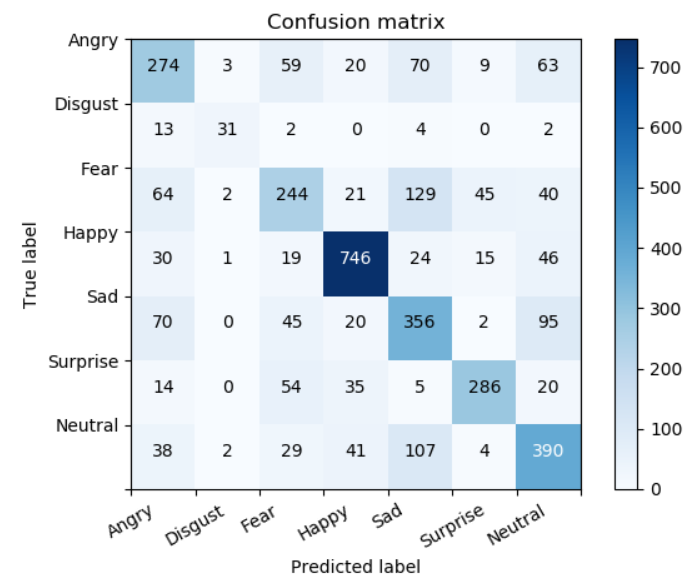
\includegraphics[width=0.8\linewidth]{confusionMatrix.png}
		}
	\end{center}
	\caption{Confusion matrix}
	\label{confusion_mat}
\end{figure}


%------------------------------------------------------------------------
\section{Proposed method}

Inferring the viewer's sentiment towards an advertisement is not trivial. As proposed in the baseline method, we can't just rely on the viewer's facial emotions alone, but we should also take into consideration other factors such as viewer's engagement and advertisement's intended motive or sentiment. In this section we will briefly describe all the components of this method, and how can they be integrated to give better results than the baseline method\ref{baselineMethod}

%-------------------------------------------------------------------------
\subsection{Facial emotion recognition} \label{FER}

The most important component is detecting the facial emotions of the viewer. For this task we can use a convolutional neural network described in the baseline approach\ref{baselineMethod}, trained on the FER dataset~\cite{FER2013}. The input to this network will be a facial landmark image, which can be obtained by the Haar feature-based cascade classifier~\cite{HaarCascade}, and the output will be a label vector containing the probabilities of each of the 7 emotions.


%-------------------------------------------------------------------------
\subsection{Viewer engagement detection} \label{VER}

Viewer's engagement plays crucial role in the experience of our approach. It is necessary to filter out viewer's emotions which are not results of the advertisement. The viewer might be talking to some other person or viewer's initial sentiment when he/she comes in the frame might be independent from her sentiment about the advertisement. Hence we are considering these external emotions as noise, and filtering those frames. To achieve this, viewer engagement detectors can be instrumented. As discussed in ~\cite{Nezami2018AutomaticRO}, we can use a convolutional neural network similar to the baseline approach\ref{baselineMethod} or VGGnet~\cite{Simonyan2014VeryDC}. For this network we will need an engagement dataset, consisting of facial data labeled with the categories engaged or disengaged.

%-------------------------------------------------------------------------
\subsection{Advertisement sentiment detection} \label{AER}

To accurately measure and quantify the viewer's reaction towards an advertisement, it is crucial to take advertisement's inherit emotion into consideration. For example, in the case of an movie poster for an horror movie should impart a scary reaction on the viewer, or an advertisement about an no-profit environmental organization having image of the burning amazon should convey a sad emotion on the viewer. These negative emotions do not mean that the viewer has a dislike for this content, but he/she is in agreement with the advertisement. The baseline approach will penalize the model in such similar cases as it will consider sad or angry to be negative emotions. To compute emotion labels for an image a simple Naive Bayes classifier can be used as presented by~\cite{ImageEmoClassification}. We can also use neural networks for this purpose, which can either be directly trained on the images or features extracted from these images such as- color, texture, composition, content as used in ~\cite{ImageEmoClassification}. Image emotion dataset~\cite{ImageEmoDataset} or IAPS dataset~\cite{IAPS} can be used for this purpose. The input to this classifier would be an advertisement poster and output will be an emotion vector describing the inherit sentiment of the advertisement.


%-------------------------------------------------------------------------
\subsection{Combining pieces}

Components described in \ref{FER}, \ref{VER} and \ref{AER} would be built and combined in the next phase of the project. The goal of the project is to build a advertisement display system which will skip or won't skip the advertisement based on the viewer's reaction towards it. The \ref{VER} component could be used to filter out noisy frames i.e. frames in which viewer is not engaged with the content. After this filtering phase, the frame could be passed to the \ref{FER} component which will give us the viewer's emotion vector. This emotion vector and an advertisement emotion vector obtained from the component \ref{AER}, can then be used to compute similarity between themselves. If this similarity is below a certain threshold, then only we will change the displayed advertisement. 
Another approach to this could be combining components \ref{AER} and \ref{FER} together into a single convolution network, which will have a softmax layer at the end with 2 neurons indicating if the advertisement should be skipped or not.

{\small
\bibliographystyle{ieee_fullname}
\bibliography{egbib}
}

\end{document}
